\documentclass[12pt,letterpaper]{article}
\usepackage[utf8]{inputenc}
\usepackage[spanish]{babel}
\usepackage{amsmath}
\usepackage{amsfonts}
\usepackage{amssymb}
\usepackage{graphicx}
\usepackage{listings}
\usepackage{hyperref}
\usepackage[left=1.5cm,right=1.5cm,top=2cm,bottom=2cm]{geometry}
\renewcommand\spanishtablename{Tabla}
\title{\textsc{Estudio de la población de México en el periodo de 1990 al 2010}}
\author{\textsc{Fabiola Vázquez}}

\begin{document}
\maketitle

\subsection*{Introducción}~\\
Se realizó un estudio de la población total por entidad federativa, de 1990 a 2010, buscando cuáles de los estados de la República Mexicana eran los más poblados. Los datos utilizados fueros extraídos de la página oficial del INEGI \cite{inegi} en un formato \textrm{xls}, exportados a \textrm{csv} y analizados con el software estadístico R versión 4.0.2 \cite{R} en el IDE \textbf{R Studio} \cite{rstudio}. 

\subsection*{Datos}~\\
Los datos descargados constan de la población total de los 32 estados de la república en el periodo 1990-2010, en saltos de 5 años. La tabla [\ref{tab:Datos}] muestra un segmento de los datos utilizados en este estudio.
\begin{table}[ht]
\centering
\begin{tabular}{rrrrrrr}
  \hline
 Estado & 1990 & 1995 & 2000 & 2005 & 2010 \\ 
  \hline
Aguascalientes & 719659 & 862720 & 944285 & 1065416 & 1184996 \\ 
 Baja California & 1660855 & 2112140 & 2487367 & 2844469 & 3155070 \\ 
 Baja California Sur & 317764 & 375494 & 424041 & 512170 & 637026 \\ 
 Campeche & 535185 & 642516 & 690689 & 754730 & 822441 \\ 
 Coahuila & 1972340 & 2173775 & 2298070 & 2495200 & 2748391 \\ 
   \hline
\end{tabular}
\caption{Parte de los datos}
\label{tab:Datos}
\end{table}

\newpage

Para analizar los datos, se hicieron diversos gráficos de caja. Además, para también tener una visualización de su distribución, añadimos gráficos de violín[\ref{violin}]. En la figura [\ref{PoblacionMexico}] se trabajó con la población total en México. Apreciamos que siempre hay al menos un valor atípico en cada gráfico de caja.

\begin{figure}[h!]
\centering

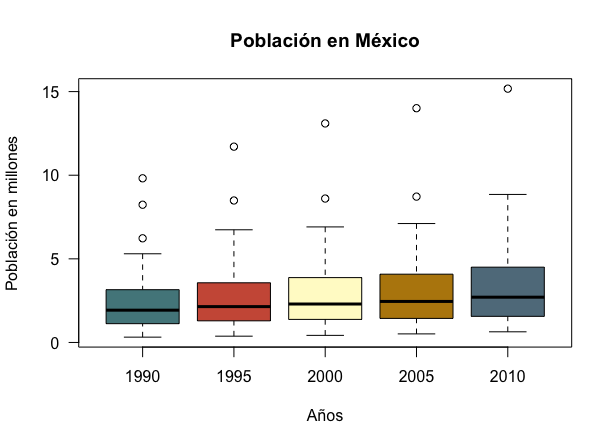
\includegraphics[scale=0.5]{Rplot02.PNG}
\caption{Gráfico de cajas de la población total en México.}
\label{PoblacionMexico}
\end{figure}

~\\

\subsection*{Resultados}~\\

 Los estados con más población son aquellos correspondientes al valor atípico alto en cada gráfico de caja, así que se realizó otro gráfico, que se visualiza en la figura [\ref{Estados}], donde observamos que los estados con mayor población son:
	\begin{enumerate}
	\item Estado de México
	\item Cd. México
	\item Veracruz
	\item Jalisco
	\item Puebla
	\item Guanajuato
	\end{enumerate}

\begin{figure}[h!]
\centering
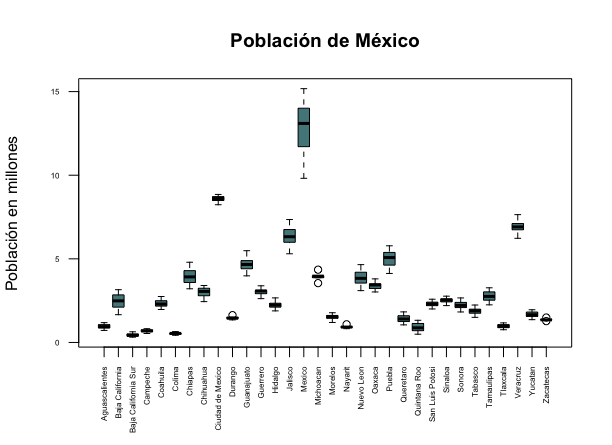
\includegraphics[scale=0.7]{estados.png}
\caption{Gráficos de caja de la población por estado.}
\label{Estados}
\end{figure}
\newpage

Para estudiar mejor los estados más poblados de México, se realiza el gráfico por separado. Como el Estado de México es el más poblado y es considerablemente más poblado que el segundo lugar, su gráfico se realizó por separado de los otros cinco más poblados, en la figura [\ref{maspoblados}].
\begin{figure}[h!]
\centering
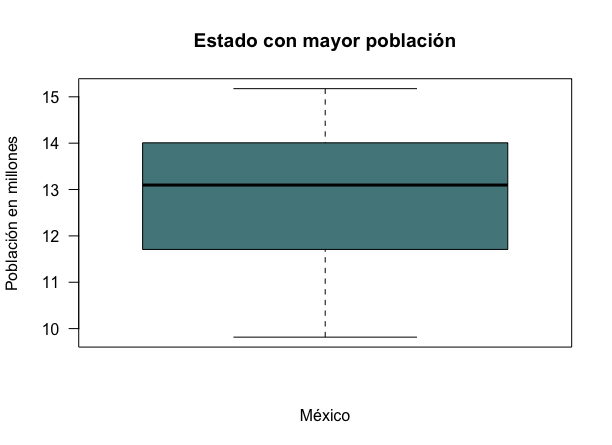
\includegraphics[scale=0.42]{mexico.png}
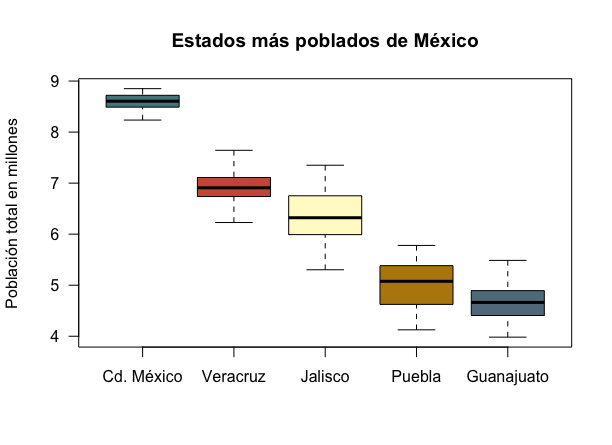
\includegraphics[scale=0.42]{mas-poblados.png}
\caption{Estados más poblados de México}
\label{maspoblados}
\end{figure}



\begin{figure}[h!]
\centering
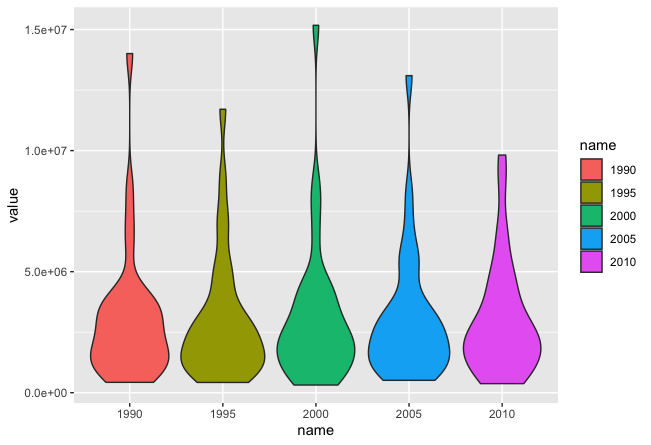
\includegraphics[scale=0.42]{violin-anos.png}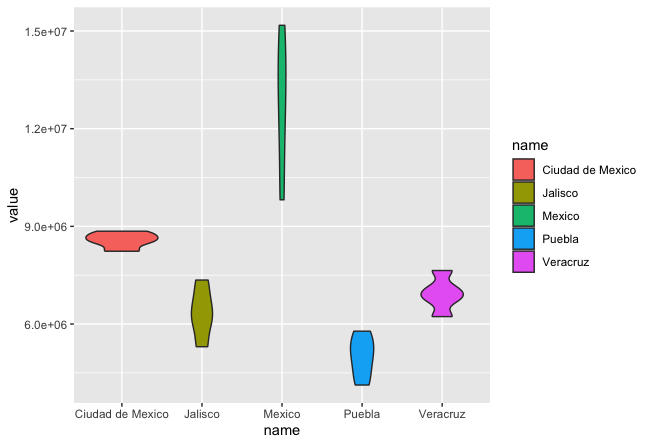
\includegraphics[scale=0.42]{violin-estados.png}
\caption{Gráficos de violín.}
\label{violin}
\end{figure}

\bibliographystyle{plain}
\bibliography{referencias}

\end{document}